% !TeX root = architecture.tex
% !TeX encoding = UTF-8
% !TeX spellcheck = en_US

\documentclass[crop,tikz]{standalone}
\usetikzlibrary{
  positioning,
  arrows,
  backgrounds,
  fit,
  calc
}

\begin{document}

% HoloClean Architecture
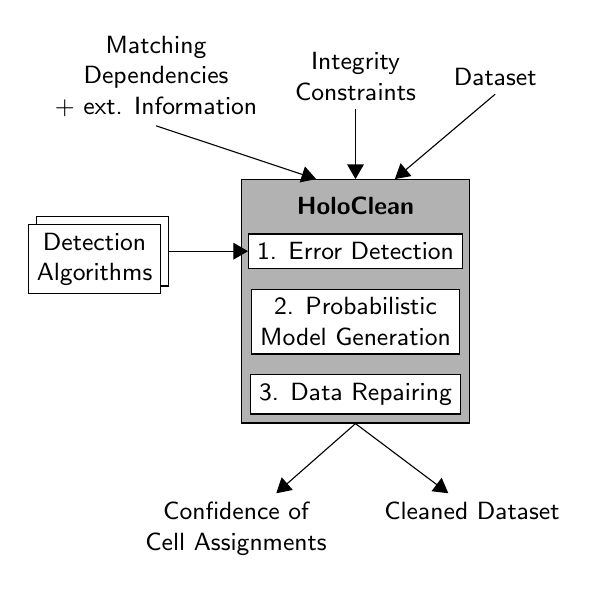
\begin{tikzpicture}[
    font=\sffamily,>=triangle 60,
    module/.style={
      draw=black,
      fill=white,
      align=center
    },
    io/.style={
      align=center
    },
    module arrow/.style={
      single arrow,
      %single arrow head extend=2.5mm,
      draw=black,
      %color=gray!20,
      shape border uses incircle,
      text height=1.5mm,
      text width=2.5mm,
      anchor=center
    }
  ]
  \small
  \newcommand{\vSep}{0.25cm}
  \newcommand{\hSep}{0.25cm}
  \newcommand{\fillColor}{black!30}
  
  % Inputs
  \node[io] (ext) {Matching\\Dependencies\\+ ext. Information};
  \node[io, right=\hSep of ext] (ics) {Integrity\\Constraints};
  \node[io, right=\hSep of ics] (dataset) {Dataset};
  
  % HoloClean
  \node[below=\vSep*4 of ics] (text) {\textbf{HoloClean}};
  \node[module, below=\vSep*.5 of text] (module1) {1. Error Detection};
  \node[module, below=\vSep of module1] (module2) {2. Probabilistic\\Model Generation};
  \node[module, below=\vSep of module2] (module3) {3. Data Repairing};
  
  \begin{scope}[name=holocleanbg, on background layer]
    \node[draw=black, fill=\fillColor, fit=(text) (module3)] (holoclean) {};
  \end{scope}
  
  % Output
  \node[io, below left=4*\vSep and \hSep of module3.south] (confidence) {Confidence of\\Cell Assignments};
  \node[io, below right=4*\vSep and \hSep of module3.south] (cleaned) {Cleaned Dataset};
  
  % I/O connections
  \draw[black,->] (dataset.south) -- ($(holoclean.north)+(0.5,0)$);
  \draw[black,->] (ics.south) -- (holoclean.north);
  \draw[black,->] (ext.south) -- ($(holoclean.north)-(0.5,0)$);
  
  \draw[black,->] (holoclean.south) -- (confidence);
  \draw[black,->] (holoclean.south) -- (cleaned);
  
  % Detection
  \node[module, left=\hSep*4 of module1,text=white] (detectors) {Detection\\Algorithms};
  \node[module, below left=1mm and 1mm of detectors.west, anchor=west] (detectors2) {Detection\\Algorithms};
  \draw[black,->] (detectors.east) -- (module1.west);
\end{tikzpicture}

\end{document}